Głównym celem każdej aplikacji cyfrowej, systemu informatycznego czy innego rodzaju usług dostępnych przez sieć jest przetwarzanie informacji cyfrowej. Dzięki dygitalizacji usług oraz utworzeniu kompletnie nowych jej, rodzajów zależnych od technologii cyfrowych ludzkość generuje masywne ilości danych każdego dnia. Jednym z najpopularniejszych środków komunikacji, zwłaszcza dla biznesu, jest poczta elektroniczna. Grupa \textbf{Radicati Inc.} spekuluje, że do końca 2023 liczba wysłanych listów elektronicznych powinna przekroczyć 347 miliardów ~\cite{radicati2019}.
\textbf{Domo, Inc}, które jest jednym z wielu dostawców usług chmurowych, w swoim raporcie zatytułowanym 
\foreignquote{english}{Data Never Sleeps 10.0} donosi o tym, że wielkość danych, które zostaną utworzone czy skopiowane może wejść w okolicę 181 zettabajtów\footnote{Zetta bajt (skrót \textbf{ZB}) w systemie SI to tryliard $10^{21}$ bajtów i $2^{70}$, czyli $1024^{7}$ bajtów.} wielkości do roku 2025 ~\cite{domo10}. Znakomita część tych danych musi być przechowywana na stałe, gdyż wymaga tego poprawne działanie systemu lub może wynikać z nakazów prawnych. Z tych powodów jednym z priorytetów przy administracji systemu jest zabezpieczenie przed utratą danych przez instytucje i działalności gospodarcze.
Do powodów utraty danych mogą należeć:
\begin{itemize}
    \item awaria nośników i innych elementów,
    \item niespodziewane braki w dostawach prądu,
    \item błąd ludzki,
    \item wirusy komputerowe.
\end{itemize}

%%%%%%%%%%%%%%%%%%%%%%%%%%%%%%%%%%%%%%%%%%%%%%%%
\section{Cel pracy}
Celem tej pracy było odnalezienie sposobu na zniwelowanie strat danych w wyniku ataku wirusa typu ransomware możliwego do wykorzystania przez administratorów w warunkach rzeczywistego ataku. Zaproponowanym przeze mnie rozwiązaniem jest oprogramowanie analizujące działania na plikach dla systemów operacyjnych z rodziny Linux.
%Celem tej pracy było utworzenie oprogramowania, które zajmuje się niwelowaniem ryzyka utraty danych z powodu ataku wirusa komputerowego typu ransomware na systemach z rodziny Linux oraz przetestowanie jego działania w trakcie rzeczywistego ataku.
 Program korzysta z informacji o stanie systemu plików i na bieżąco analizuje wykonywane na nim operacje. Statystyki z obserwowanego obszaru zawierają w sobie m.in. ilości operacji, ścieżkę do użytej komendy, nazwę użytkownika, który dokonuje operacji etc. Dzięki temu administrator może nie tylko dowiedzieć się o potencjalnym zagrożeniu ataku ransomware, ale też obserwować dowolny, podejrzany ruch na systemie plików. Następnie dokonywana jest analiza zawartości plików i generowany jest raport o zakresie ryzyka.
Docelową grupą użytkowników są administratorzy, a więc główne założenia, jakie postawiłem sobie w trakcie tworzenia rozwiązania, miały na celu wytworzenie oprogramowania łatwego dla nich w obsłudze. Tymi założeniami są:
\begin{itemize}
    \item łatwa instalacja, która nie wymaga aktualizacji sterowników sprzętowych,
    \item wsparcie dla najpopularniejszych dystrybucji serwerowych\footnote{W3 Techs utrzymuje raport o sieciowych serwerach Linuksowych. Jest on codziennie aktualizowany i można go odnaleźć pod adresem: https://w3techs.com/technologies/details/os-linux},
    \item minimalne zużycie zasobów,
    \item integracja z bieżącymi popularnymi rozwiązaniami w administracji systemów.
\end{itemize}

%%%%%%%%%%%%%%%%%%%%%%%%%%%%%%%%%%%%%%%%%%%%%%%%
\section{Opis problemu i znaczenie zagrożeń typu ransomware}
 Od 2017 roku obserwuje się trend wzrostowy ataków ransomware~\cite{petrosyan_worldwide_nodate}, a w ciągu pierwszej połowy 2022 roku, dokonano 236,7 miliona ataków na całym świecie 
 ~\cite{petrosyan_number_nodate}. Wg. raportu Verizona \footnote{Raport jest odpłatnie dostępny pod linkiem: https://www.verizon.com/business/resources/reports/dbir/2021/results-and-analysis} ataki ransomware stanowią 10\% wszystkich naruszeń danych w 2021. Wedle zebranych statystyk wykrycie ich zajęło w aż 49 dni dłużej niż średni czas wykrycia wszystkich naruszeń z tego samego roku. Raport wyjaśnia też, że zagrożona nie jest wyłącznie branża IT, ale też inne sektory, w szczególności sektor ochrony zdrowia.
\begin{figure}[H]
     \centering
     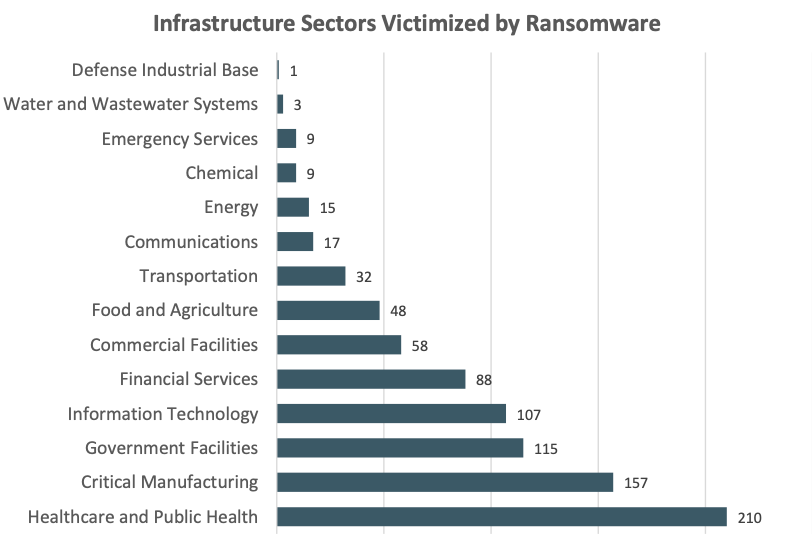
\includegraphics[width=0.78\linewidth]{rysunki/attacks_on_sectors.png}
     \caption{Sektory infrastruktury krytycznej, do których odnosiły się skargi IC3. Źródło: \emph{FBI 2022 Internet Crime Report}, s. 14}
     \label{fig:enter-label}
 \end{figure}
 Raport IC3 z roku 2022 donosi o 870 zarejestrowanych skargach dotyczących ataków, których celem były organizacje infrastruktury krytycznej. Pośród 16 sektorów, 14 z nich padło ofiarą próby ataku.
  \begin{figure}[H]
     \centering
     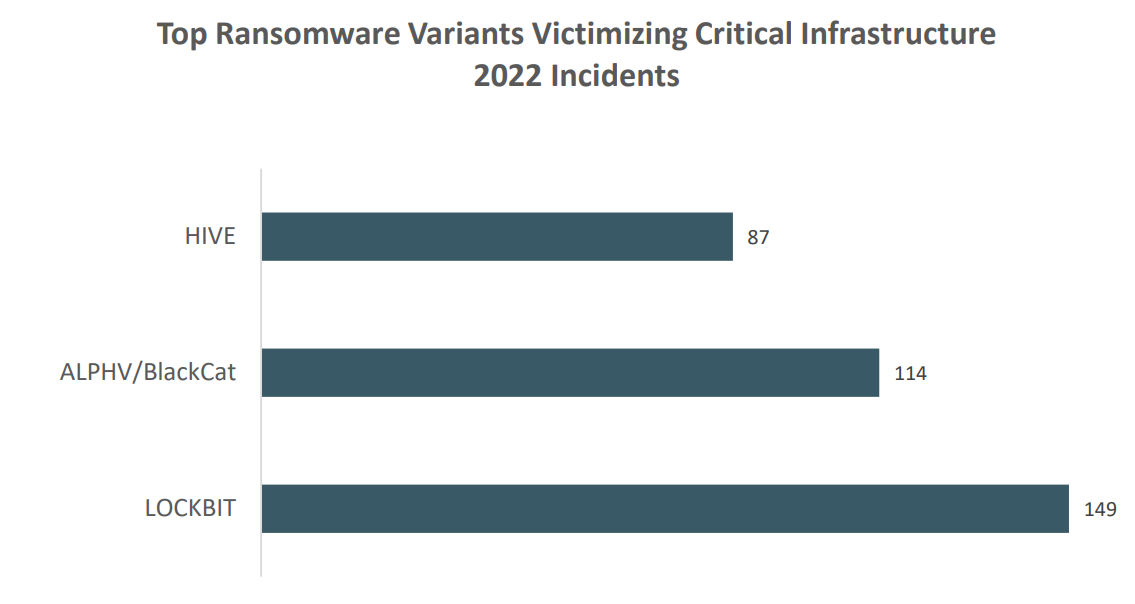
\includegraphics[width=0.75\linewidth]{rysunki/topransomwares2022.png}
     \caption{Najpopularniejsze warianty wirusów ransomware, zarejestrowane w trakcie incydentów mających na celu atak infrastruktury krytycznej. Należy zauważyć, że wirus \foreignquote{english}{LockBit} sprawiał najwięcej problemów. Jego wersja na system Linux nosi nazwę \foreignquote{english}{LockBit Linux-ESXi Locker }. Źródło: \emph{FBI 2022 Internet Crime Report}, s. 15}
     \label{fig:enter-label}
 \end{figure}
 Raport grupy \foreignquote{english}{Herjavec} donosi, że aż 70\% organizacji medycznych borykało się z poważnymi komplikacjami przez ataki ransomware ~\cite{health}.
 W 2022 roku 1 na 42 instytucje ochrony zdrowia były ofiarami tychże ataków, 74\% z nich to szpitale 
 ~\cite{etal_check_2022}.
 \begin{figure}[H]
    \centering
    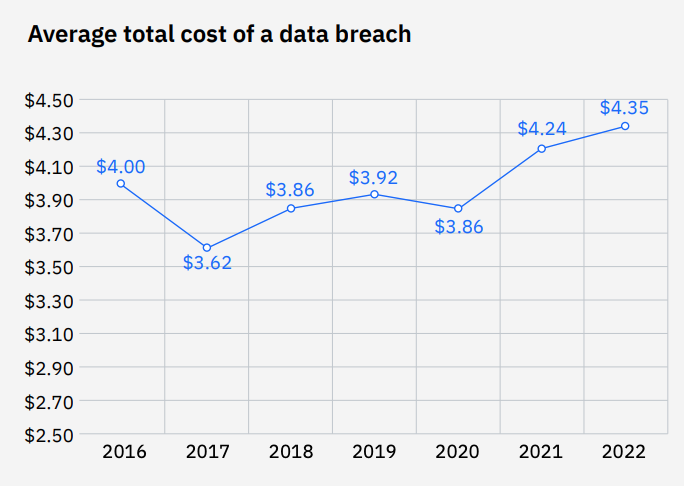
\includegraphics[width=0.7\linewidth]{rysunki/costOfDataBreach.png}
    \caption{Średni koszt naruszenia danych 2016-2022. Źródło: \emph{Cost of a Data Breach
Report 2022}, figure 1, s. 9.}
    \label{fig:enter-label}
\end{figure}
 Z danych zebranych z ostatnich 5 lat jednoznacznie wynika, że nieumiejętne przeciwdziałanie może zaszkodzić nie tylko finansom zaatakowanej działalności lub osoby indywidualnej, ale również stwarza zagrożenie dla zdrowia i życia.
 Dodatkowo, mając na uwadze średni koszt naruszenia danych w 2023, którego globalna średnia wynosi 4,45 milionów USD ~\cite{petrosyan_global_cost},
 coraz więcej administratorów jest zmuszonych dywersyfikować sposoby zabezpieczania systemów. 
 \begin{figure}[H]
     \centering
     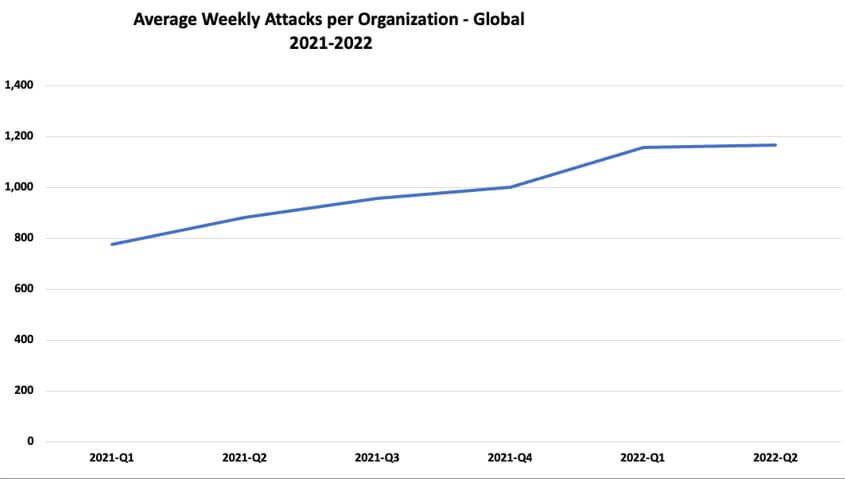
\includegraphics[width=0.75\linewidth]{rysunki/Global-Quarterly-attacks-from-Q1-2021- Q2-2022.png}
     \caption{Globalnie zgłoszone incydenty ataków ransomware per kwartał w roku 2022 zarejestrowanych przez Check Point Research. Organizacja spekuluje, że wzrost ataków mógł być spowodowany lukami bezpieczeństwa \foreignquote{english}{log4j} oraz cyberataków związanych z wojną w Ukrainie. Źródło: \emph{Check Point Research: Weekly Cyber Attacks increased by 32\% Year-Over-Year; 1 out of 40 organizations impacted by Ransomware}, figure 1.}
     \label{fig:enter-label}
 \end{figure}
 Na rynku istnieje wiele popularnych rozwiązań działających prewencyjnie m.in. w tym rozbudowane aplikacje służące do tworzenia i przywracania kopii zapasowych. Należy jednak wziąć pod uwagę, że przywracanie danych nie jest prostym procesem. W zależności od rodzaju użytego nośnika przywracanie może doprowadzić nawet do przypadkowej utraty danych przy zniszczeniu nośnika danych w przypadku taśm. Jest to także proces powolny, co w efekcie może spowodować poniesienie większych kosztów niż wartość okupu.
 \newline
 Rozwiązaniem, które wydaje się być aktualnie najlepszym, jest możliwie jak najwcześniejsze wykrycie potencjalnego źródła ataku. W przypadku, gdy te czynności zawiodą, jedyną możliwością na zmniejszenie strat jest minimalizacja skutków ataku na bieżąco. Aby tego dokonać, konieczne jest wczesne wykrycie ataku.
 
\begin{figure}[H]
\centering
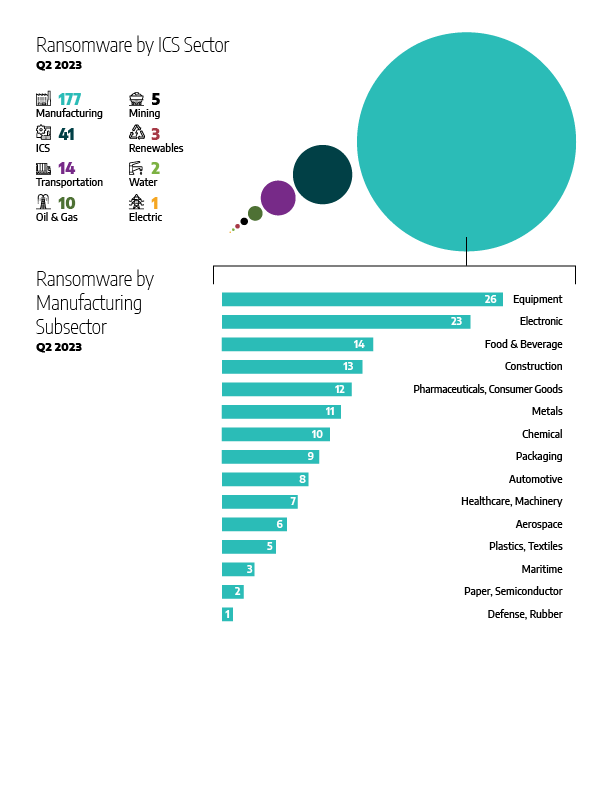
\includegraphics[width=0.6\linewidth]{rysunki/attackbysector.png}
\caption{Incydenty ransomware per sektor gospodarki. Źródło: \emph{Dragos Industrial Ransomware Attack Analysis: Q2 2023}, figure 2.}
\label{fig:enter-label}
\end{figure}
 


%%%%%%%%%%%%%%%%%%%%%%%%%%%%%%%%%%%%%%%%%%%%%%%%
\section{Krótka charakterystyka ataków ransomware}
Ransomware można zdefiniować jako oprogramowanie, które blokuje atakowanemu dostęp do danych, do momentu zapłacenia okupu ~\cite{ransomware_us}. Prostsze ataki mogą sprowadzać się do blokady systemu bez uszkadzania plików, jednak większym zagrożeniem są tzw. \foreignquote{english}{cryptovirological attacks} ~\cite{502676}, czyli ataki wykorzystujące szyfrowanie danych jako formę blokady danych. Atakowany, jeśli nie posiada kopii zaszyfrowanych danych, musiałby odnaleźć klucz, którego użyto w szyfrowaniu. Nawet jeśli atakowany wie jakiego algorytmu użyto w ataku, to odnalezienie klucza jest problemem trudnym, zwłaszcza dla nowoczesnych algorytmów szyfrowania. Przykładowo, algorytm \foreignquote{english}{AES} w zależności od klucza występuje w wariantach 128,192 oraz 256-bitowych, co daje między $2^{128}$ a $2^{256}$ możliwych wartości do sprawdzenia atakiem siłowym. 
\newline
Przy wyłudzaniu okupu, atakujący stosują również techniki zastraszenia. Przykładowo wirus \foreignquote{english}{WannaCry}, którego duża fala ataków miała miejsce w 2017 roku ~\cite{czarnecki_oto_2017}, informował, że początkowy okup 300\$ per maszyna wzrośnie dwukrotnie po 3 dobach zwłoki. Po upływie tygodnia odzyskanie danych miałoby stać się niemożliwe. Atakujący wymagają, aby okup został spłacony w sposób trudny do wyśledzenia przez organy ścigania m.in. za pomocą kryptowalut.
\begin{figure}[H]
    \centering
    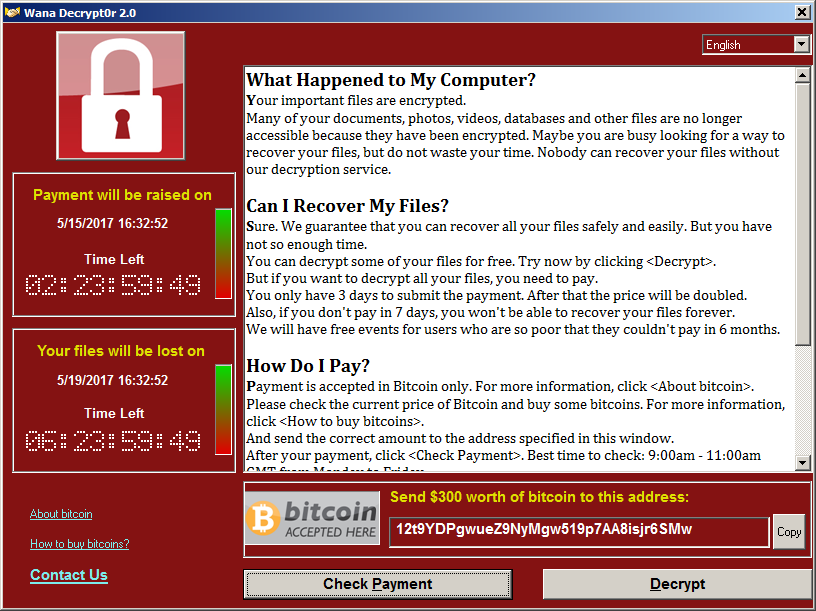
\includegraphics[width=0.95\linewidth]{rysunki/wannacry.png}
    \caption{Ekran wyświetlający się po zainfekowaniu komputera przez WannaCry. Atakujący wymaga od ofiary zapłaty Bitcoinem.}
    \label{fig:enter-label}
\end{figure}

Ataki ransomware, mogą także założyć blokadę powłoki systemowej lub nawet dokonać modyfikacji partycji rozruchu jak w przypadku wirusa RedBoot ~\cite{redboot}.

\begin{figure}[H]
    \centering
    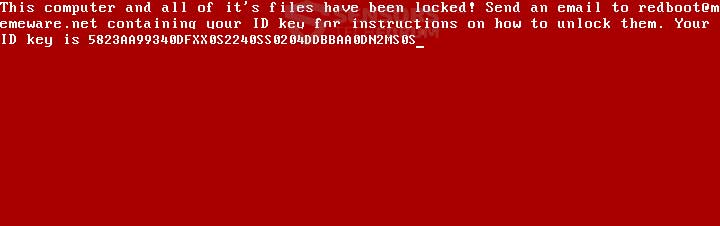
\includegraphics[width=0.95\linewidth]{rysunki/redboot.png}
    \caption{Ekran rozruchu przy infekcji wirusem RedBoot.}
    \label{fig:enter-label}
\end{figure}

Konceptualnie \foreignquote{english}{cryptovirological attack} został przedstawiony w 1996 roku na konferencji IEEE Security \& Privacy~\cite{yung}. Opisuje się go jako protokół pomiędzy atakowanym, a atakującym:

\begin{figure}[H]
    \centering
    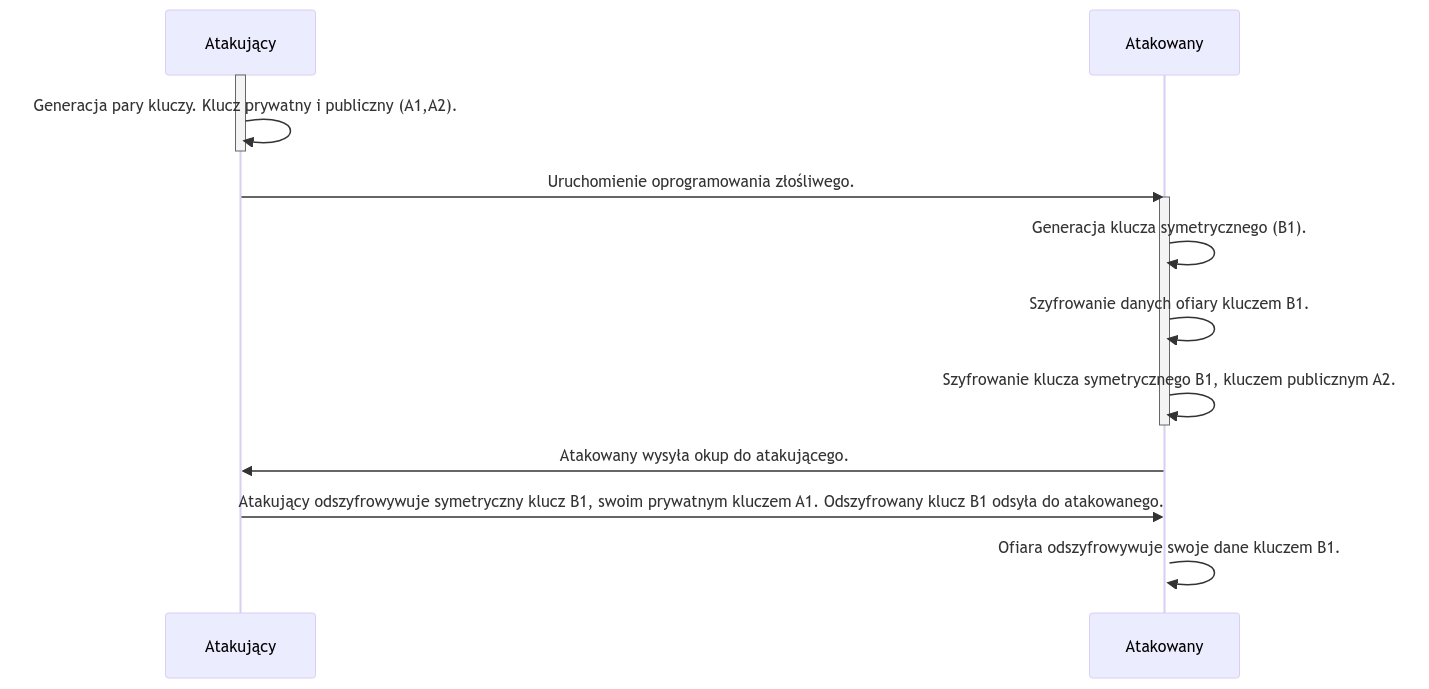
\includegraphics[width=1\linewidth]{rysunki/sequenceRansomware.png}
    \caption{Diagram sekwencji ataku ransomware.}
    \label{fig:enter-label}
\end{figure}
Generowany klucz symetryczny ma charakter losowy i nie pomoże w odszyfrowaniu danych innej ofiary. Klucz prywatny jest przechowywany wyłącznie przez atakującego. Jedyny kontakt, jaki musi być wykonany bezpośrednio przez atakującego, następuje w momencie kiedy zaszyfrowany klucz symetryczny jest wysyłany do atakującego, a następnie klucz odszyfrowany do atakowanego.
\newline
Typowymi sposobami propagacji ransomware są:
\begin{itemize}
    \item podszywanie się pod znane aplikacje czy strony internetowe,
    \item skuszenie ofiary do otworzenia niezaufanego załącznika listu elektronicznego,
    \item luki bezpieczeństwa sieci.
\end{itemize}

%%%%%%%%%%%%%%%%%%%%%%%%%%%%%%%%%%%%%%%%%%%%%%%%